
In addition to the law-big, the investigation into the suitability of Ampersand also covers the list of regulations (see list ~\ref{list:ass-laws-regulations}.
Due to time-boxing it is not possible to analyze and process all associated laws and regulations.
The aim is not to provide a fully elaborated conceptual analysis, but to test Ampersand for usability.

%The results of the study will be discussed in the following sections.
%The research that focuses on the research question "\acrlong{research question}".
%By answering the derived questions, we provide a view on the usability of Ampersand.

To test the usability of Ampersand, we collected information about things that stood out while building the prototype.
This information is included as observations in appendix~\ref{appendixLoglines}.

The first classification of the observations was made according to the sub-questions.
Assuming that this would provide answers about the sub-questions, which in turn lead to claims regarding the main question.
For each observation, the core of the observation is also indicated.
Given the roughness of the material, it was sometimes possible to indicate several cores per observation.

This categorization has resulted in counts per key concept.
The numbers give an idea of where the most attention was paid during the observation.

\begin{comment}
Deductief redeneren is een top-down onderzoeksmethode. Je zoekt op basis van een generalisatie naar specifieke gevallen. Met behulp van deductief onderzoek toets je theorieën en hypothesen. Het proces bestaat over het algemeen uit vier stappen: er is een theorie (generalisering), je formuleert een hypothese, je observeert of analyseert, je bevestigt of verwerpt de hypothese.
\end{comment}
The approach chosen is the qualitative content analysis method of \cite{mayring_qualitative_2019}.
Specific cases that support the generalization are sought on the basis of generalizations.
We conduct a top-down investigation by means of deductive reasoning.

We then work with pre-formulated categories, which are derived from the main question.
And establish the relationship between the categories and the observations.
This step consists of a methodologically controlled assignment of the category to a text passage of the observation.
This then leads to a deductive approach.
\begin{figure}[H]
    \centering
    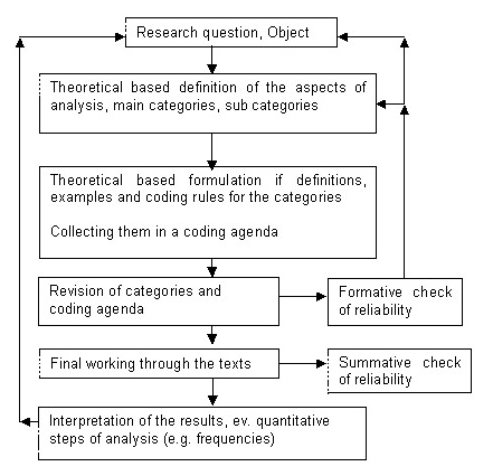
\includegraphics{Step model of deductive category application.PNG}
    \caption{Step model of deductive category application\citep{mayring_qualitative_2000}}
    \label{fig:step-model-of-deductive-category-application}
\end{figure}

The starting point is that the usability of Ampersand is an issue.
We see this because Ampersand is rarely used.
We hypothesize that we can determine the cause of the low usage through research.
The research therefore focuses on the following main question, \acrlong{research question}.

While making the prototype, we record what we notice.
The record is tagged with an initial assignment to the sub-question and the date and time of the observation.
So that the observation remains traceable.
And we hold discussions with stakeholders in the form of free interviews.

Given the nature of the notes, the choice is for deductive categories\citep{mayring_qualitative_2019}.
Based on the main question, we cluster according to the terms of the main question (see list \ref{list:deductive-categrories}, \nameref{list:deductive-categrories}).
The main question is linked to this project and the categories from this list are added.
For each category it is defined what the observations and interview report paragraphs must meet.
We use the following definitions for the assignment.
\begin{table}[H]
    \begin{tabularx}{\linewidth}{|X|X|}
    \hline
        \textbf{Category} & \textbf{Definition} \\\hline
        \acrshort{cat1} & \acrlong{cat1} \\\hline
        \acrshort{cat2} & \acrlong{cat2} \\\hline
        \acrshort{cat3} & \acrlong{cat3} \\\hline
        \acrshort{cat4} & \acrlong{cat4} \\\hline
        \acrshort{cat5} & \acrlong{cat5} \\\hline
        \acrshort{cat6} & \acrlong{cat6} \\\hline
        \acrshort{cat7} & \acrlong{cat7} \\\hline
    \end{tabularx}
    \caption{Category definitions}
    \label{tab:Category definitions}
\end{table}

We determine the coding rules for each category and, if necessary, also provide an example.
We then work through the observations and determine to which category the text belongs.
Here we use our chosen identification of observation.
The interview reports are divided into paragraphs and we determine to which category the paragraph belongs.
We use a textual reference to the text here.
By means of a loop-back the theoretical basis can be further refined as can be seen in figure \ref{fig:step-model-of-deductive-category-application}.

Philip Mayring is also the founder of the website \url{https://www.qcamap.org}.
The content analysis tool on the said website allows us to perform part of the content analysis.
We define a project within QCAMap, the working method is linked to this project.
For our research the deductive approach.

In the next section, section~\ref{Discussion} the interpretations of the results will be discussed.







